%% This is the ctufit-thesis example file. It is used to produce theses
%% for submission to Czech Technical University, Faculty of Information Technology.
%%
%% This is version 1.3.10, built 27. 2. 2025.
%% 
%% Get the newest version from
%% https://gitlab.fit.cvut.cz/theses-templates/FITthesis-LaTeX
%%
%%
%% Copyright 2024, Tomas Novacek
%% Copyright 2021, Eliska Sestakova and Ondrej Guth
%%
%% This work may be distributed and/or modified under the
%% conditions of the LaTeX Project Public License, either version 1.3
%% of this license or (at your option) any later version.
%% The latest version of this license is in
%%  https://www.latex-project.org/lppl.txt
%% and version 1.3 or later is part of all distributions of LaTeX
%% version 2005/12/01 or later.
%%
%% This work has the LPPL maintenance status `maintained'.
%%
%% The current maintainer of this work is Tomas Novacek (novacto3@fit.cvut.cz).
%% Alternatively, submit bug reports to the tracker at
%% https://gitlab.fit.cvut.cz/theses-templates/FITthesis-LaTeX/issues
%%
%%

% arara: xelatex
% arara: biber
% arara: xelatex
% arara: xelatex

%%%%%%%%%%%%%%%%%%%%%%%%%%%%%%%%%%%%%%%%%
% CLASS OPTIONS
% language: czech/english/slovak
% thesis type: bachelor/master/dissertation
% colour: bw for black&white OR no option for default colour scheme
% electronic (oneside) or printed (twoside), twoside is default
% paragraph - if passed, this optional argument sets paragraphs as the deepest level of headers, styles it, numbers it and adds it to Table of Content. Use with care! Normally, it is considered unwise to use it, since its too deep.
%%%%%%%%%%%%%%%%%%%%%%%%%%%%%%%%%%%%%%%%%
\documentclass[czech,bachelor,unicode,oneside]{ctufit-thesis}

%%%%%%%%%%%%%%%%%%%%%%%%%%%%%%%%%%
% FILL IN THIS INFORMATION
%%%%%%%%%%%%%%%%%%%%%%%%%%%%%%%%%%
\ctufittitle{Název příkladné závěrečné práce} % replace with the title of your thesis
\ctufitauthorfull{Bc. Jiří Nebozíz} % replace with your full name (first name(s) and then family name(s) / surname(s)) including academic degrees
\ctufitauthorsurnames{Nebozíz} % replace with your surname(s) / family name(s)
\ctufitauthorgivennames{Jiří} % replace with your first name(s) / given name(s)
\ctufitsupervisor{doc.\,Ing.\,Damien Zlo,\,Ph.D.} % replace with name of your supervisor/advisor (include academic degrees)
\ctufitdepartment{Katedra teoretické informatiky} % replace with the department of your defence
\ctufityear{2021} % replace with the year of your defence
\ctufitdeclarationplace{Praze} % replace with the place where you sign the declaration
\ctufitdeclarationdate{\today} % replace with the date of signature of the declaration
\ctufitabstractCZE{Fill in the abstract of this thesis in Czech. Lorem ipsum dolor sit amet. Class aptent taciti sociosqu ad litora torquent per conubia nostra, per inceptos hymenaeos. Cras pede libero, dapibus nec, pretium sit amet, tempor quis. Sed vel lectus. Donec odio tempus molestie, porttitor ut, iaculis quis, sem. Suspendisse sagittis ultrices augue.}
\ctufitabstractENG{Fill in the abstract of this thesis in English. Lorem ipsum dolor sit amet. Class aptent taciti sociosqu ad litora torquent per conubia nostra, per inceptos hymenaeos. Cras pede libero, dapibus nec, pretium sit amet, tempor quis. Sed vel lectus. Donec odio tempus molestie, porttitor ut, iaculis quis, sem. Suspendisse sagittis ultrices augue.}
\ctufitkeywordsCZE{enter, comma, separated, list, of, keywords, in, CZECH}
\ctufitkeywordsENG{enter, comma, separated, list, of, keywords, in, ENGLISH}
%%%%%%%%%%%%%%%%%%%%%%%%%%%%%%%%%%
% END FILL IN
%%%%%%%%%%%%%%%%%%%%%%%%%%%%%%%%%%

%%%%%%%%%%%%%%%%%%%%%%%%%%%%%%%%%%
% CUSTOMIZATION of this template
% Skip this part or alter it if you know what you are doing.
%%%%%%%%%%%%%%%%%%%%%%%%%%%%%%%%%%

\RequirePackage{iftex}[2020/03/06]
\iftutex % XeLaTeX and LuaLaTeX
    \RequirePackage{ellipsis}[2020/05/22] %ellipsis workaround for XeLaTeX
\else
    \errmessage{Only compilation with XeLaTeX or LuaLaTeX is allowed}
    \stop
\fi

% hyperlinks
\hypersetup{
    pdfpagelayout=TwoPageRight,
    colorlinks=false,
    allcolors=decoration,
    pdfborder={0 0 0.1}
}

% uncomment the following to hide all hyperlinks
%\hypersetup{hidelinks}

% uncomment the following to change the colour of all hyperlinks to CTU blue
%\hypersetup{allbordercolors=decoration}

\RequirePackage{pdfpages}[2020/01/28]

%%%%%%%%%%%%%%%%%%%%%%%%%%%%%%%%%%
% CUSTOMIZATION of this template END
%%%%%%%%%%%%%%%%%%%%%%%%%%%%%%%%%%


%%%%%%%%%%%%%%%%%%%%%%
% PACKAGES SETTINGS
% You may choose to modify this part.
%%%%%%%%%%%%%%%%%%%%%%
\usepackage{dirtree}
\usepackage{lipsum,tikz}
\usepackage[style=iso-numeric]{biblatex}
\addbibresource{text/bib-database.bib}
\usepackage{xurl}
\usepackage{listings} % typesetting of sources
%\usepackage{minted}
\usepackage{csquotes}

%%%%%%%%%%%%%%%%%%%%%%
% PACKAGES SETTINGS END
%%%%%%%%%%%%%%%%%%%%%%

\begin{document} 
\frontmatter\frontmatterinit % do not remove these two commands

\thispagestyle{empty}\maketitle\thispagestyle{empty}\cleardoublepage % do not remove these four commands

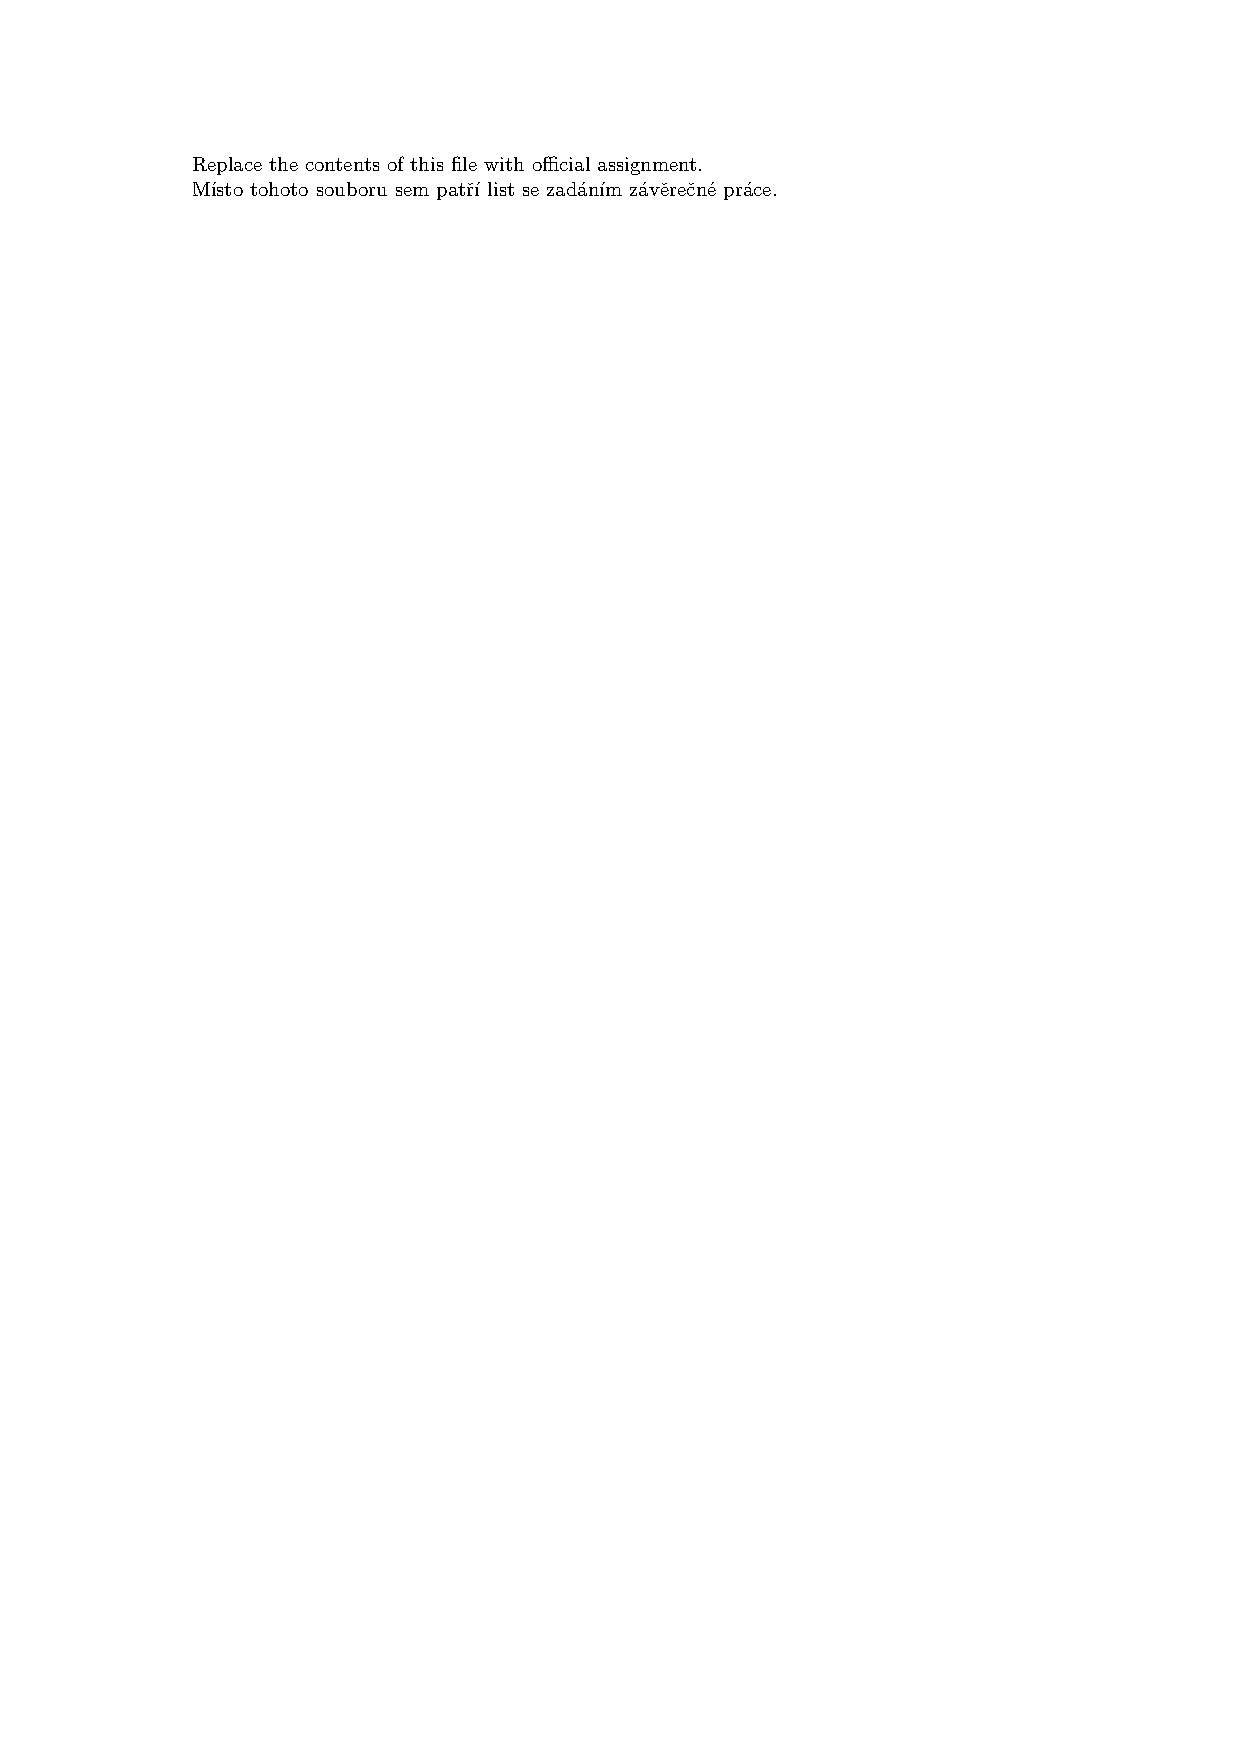
\includepdf[pages={1-}]{example-assignment-include.pdf} % replace this file with your thesis assignment generated from ProjectsFIT

\imprintpage % do not remove this command
\stopTOCentries
%%%%%%%%%%%%%%%%%%%%%%
% list of other contents END
%%%%%%%%%%%%%%%%%%%%%%

%%%%%%%%%%%%%%%%%%%
% ACKNOWLEDGMENT
% FILL IN / MODIFY
% This is a place to thank people for helping you. It is common to thank your supervisor.
%%%%%%%%%%%%%%%%%%%
\begin{acknowledgmentpage}
	Chtěl bych poděkovat především sit amet, consectetuer adipiscing elit. Curabitur sagittis hendrerit ante. Class aptent taciti sociosqu ad litora torquent per conubia nostra, per inceptos hymenaeos. Cras pede libero, dapibus nec, pretium sit amet, tempor quis. Sed vel lectus. Donec odio tempus molestie, porttitor ut, iaculis quis, sem. Suspendisse sagittis ultrices augue.
\end{acknowledgmentpage} 
%%%%%%%%%%%%%%%%%%%
% ACKNOWLEDGMENT END
%%%%%%%%%%%%%%%%%%%


%%%%%%%%%%%%%%%%%%%
% DECLARATION
% FILL IN / MODIFY
%%%%%%%%%%%%%%%%%%%
% INSTRUCTIONS
% ENG: choose one of approved texts of the declaration. DO NOT CREATE YOUR OWN. Find the approved texts at https://courses.fit.cvut.cz/SFE/download/index.html#_documents (document Declaration for FT in English)
% CZE/SLO: Vyberte jedno z fakultou schvalenych prohlaseni. NEVKLADEJTE VLASTNI TEXT. Schvalena prohlaseni najdete zde: https://courses.fit.cvut.cz/SZZ/dokumenty/index.html#_dokumenty (prohlášení do ZP)
\begin{declarationpage}
FILL IN ACCORDING TO THE INSTRUCTIONS. VYPLŇTE V SOULADU S POKYNY. Lorem ipsum dolor sit amet, consectetuer adipiscing elit. Curabitur sagittis hendrerit ante. Class aptent taciti sociosqu ad litora torquent per conubia nostra, per inceptos hymenaeos. Cras pede libero, dapibus nec, pretium sit amet, tempor quis. Sed vel lectus. Donec odio tempus molestie, porttitor ut, iaculis quis, sem. Suspendisse sagittis ultrices augue. Donec ipsum massa, ullamcorper in, auctor et, scelerisque sed, est. In sem justo, commodo ut, suscipit at, pharetra vitae, orci. Pellentesque pretium lectus id turpis.

Lorem ipsum dolor sit amet, consectetuer adipiscing elit. Curabitur sagittis hendrerit ante. Class aptent taciti sociosqu ad litora torquent per conubia nostra, per inceptos hymenaeos. Cras pede libero, dapibus nec, pretium sit amet, tempor quis. Sed vel lectus. Donec odio tempus molestie, porttitor ut, iaculis quis, sem. Suspendisse sagittis ultrices augue. Donec ipsum massa, ullamcorper in, auctor et, scelerisque sed, est. In sem justo, commodo ut, suscipit at, pharetra vitae, orci. Pellentesque pretium lectus id turpis.
\end{declarationpage}
%%%%%%%%%%%%%%%%%%%
% DECLARATION END
%%%%%%%%%%%%%%%%%%%

\printabstractpage % do not remove this command

%%%%%%%%%%%%%%%%%%%
% SUMMARY
% FILL IN / MODIFY
% OR REMOVE ENTIRELY (upon agreement with your supervisor)
% (appropriate to remove in most theses)
%%%%%%%%%%%%%%%%%%%
% \begin{summarypage}
% \section*{Summary section}
% 
% \lipsum[1][1-8]
% 
% \section*{Summary section}
% 
% \lipsum[2][1-6]
% 
% \section*{Summary section}
% 
% \lipsum[3]
% 
% \section*{Summary section}
% 
% \lipsum[2]
% 
% \section*{Summary section}
% 
% \lipsum[1][1-8] Lorem lorem lorem.
% \end{summarypage}
%%%%%%%%%%%%%%%%%%%
% SUMMARY END
%%%%%%%%%%%%%%%%%%%

\tableofcontents % do not remove this command
%%%%%%%%%%%%%%%%%%%%%%
% list of other contents: figures, tables, code listings, algorithms, etc.
% add/remove commands accordingly
%%%%%%%%%%%%%%%%%%%%%%
\listoffigures % list of figures
\begingroup
\let\clearpage\relax
\listoftables % list of tables. Remove if you do not have any.
\thectufitlistingscommand % list of code listings. Remove if you do not have any.
\endgroup

%%%%%%%%%%%%%%%%%%%
% ABBREVIATIONS
% FILL IN / MODIFY
% OR REMOVE ENTIRELY
% List the abbreviations in lexicography order.
%%%%%%%%%%%%%%%%%%%
\chapter{\thectufitabbreviationlabel}
	
\begin{tabular}{rl}
DFA & Deterministic Finite Automaton\\
FA & Finite Automaton\\
LPS & Labelled Prüfer Sequence\\
NFA & Nondeterministic Finite Automaton\\
NPS & Numbered Prüfer Sequence\\
XML & Extensible Markup Language\\
XPath & XML Path Language\\
XSLT & eXtensible Stylesheet Language Transformations\\
W3C & World Wide Web Consortium
\end{tabular}
%%%%%%%%%%%%%%%%%%%
% ABBREVIATIONS END
%%%%%%%%%%%%%%%%%%%
\resumeTOCentries
\mainmatter\mainmatterinit % do not remove these two commands
%%%%%%%%%%%%%%%%%%%
% THE THESIS
% MODIFY ANYTHING BELOW THIS LINE
%%%%%%%%%%%%%%%%%%%

% Do not forget to include Introduction
%---------------------------------------------------------------
\chapter{Úvod}
% uncomment the following line to create an unnumbered chapter
%\chapter*{Introduction}\addcontentsline{toc}{chapter}{Introduction}\markboth{Introduction}{Introduction}
%---------------------------------------------------------------
\setcounter{page}{1}

% The following environment can be used as a mini-introduction for a chapter. Use that any way it pleases you (or comment it out). It can contain, for instance, a summary of the chapter. Or, there can be a quotation.
 %\begin{chapterabstract}
%	\lipsum[1]
%\end{chapterabstract}

%\lipsum[2][1-4]{} [1]

%\lipsum[4]

Se zvyšujícím se počtem obyvatel Země se zvyšuje i poptávka po mobilitě, což vede k nárůstu množství dopravních prostředků.
Větší hustota dopravy sebou ale přináší nevýhody. S rostoucím počtem dopravních prostředků stoupá i množství nehod, klesá rychlost a efektivita dopravy a s tím je spojené i větší znečištění životního prostředí.

Proto je důležité vyvíjet a využívat technologie, které se těmito problémy zabývají. Jednou z těchto technologií je právě V2X (Vehicle-to-everything) komunikace.
Hlavními cíli V2X je zvýšit bezpečnost, efektivitu
a umožnit tak udržitelný růst silničního provozu. Vedlejším, ale neméně důležitým
cílem, je také snížení dopadu dopravy na životní prostředí, právě zvýšením
efektivity.

Součástí V2X jsou různé standardy popisující komunikaci mezi několika druhy zařízení
(vozidlo – vozidlo, vozidlo – zařízení infrastruktury) a různé V2X zprávy.
Moje práce se zaměřuje hlavně na zprávy CAM (Coop awarenes message)
a DENM (Decentralized enviromental message).

V2X zprávy jsou kódované pomocí Abstract Syntax Notation One (ASN.1), nástroje pro kódování abstraktních datových struktur. Na překlad ASN.1 specifikací a dekódování V2X zpráv se soustředí první část mojí práce.

Komunikace V2X i standardy používané pro její kódování (ASN.1) existují
již řadu let, proto jsou již dostupné různé komerční i opensource překladače
a dekodéry. Hlavním cílem mé práce je porovnat dostupná řešení, vybrat z nich
nejlépe udržované a dobře použitelné projekty, hlavně ASN.1 kompilátor, a s jejich
pomocí vytvořit aplikaci pro dekódování a vizualizaci CAM a DENM zpráv.

Moje motivace pro dané téma vychází z několika důvodů. Prvním jsou použité
technologie, s prací v prostředí .NET mám již kladné zkušenosti a chci
se jí tak věnovat v budoucnu. Dalším důvodem je, že vyvíjená aplikace může
mít hned po dokončení práce reálné využití. Posledním důvodem je budoucnost
řešené problematiky, podle mého názoru bude V2X komunikace v blízké
budoucnosti jedině růst a práce tak zůstane aktuální.

%===============================================================================
\chapter{Cíl práce}

Tato bakalářská práce se dá rozdělit na několik navazujících částí.

Prvním cílem mojí práce, je navrhnout architekturu v prostředí .NET, která bude vhodná pro překlad a dekódování. Architekturou je myšlena struktura a rozvržení C# tříd, které budou odpovídat zadaným ASN.1 specifikacím a budou generované kompilátorem.

Dalším cílem je nalezení nebo vytvoření programu, který bude překládat ASN.1 specifikace do zdrojového kódu v jazyce C#. Psaní celého kompilátoru není záměrem práce, proto se v této části zabývám nejprve výběrem vhodného kompilátoru, schopného zpracovávat potřebné ASN.1 specifikace pro zadané V2X zprávy a poté případným dopsáním funkcí nebo jeho úpravou, tak, aby výsledný program generoval zdrojový kód v jazyce C#.

Třetí část práce se zaměřuje na dekódování ASN.1 zpráv. Tato část přímo navazuje na část první, dekodér pro práci využívá zdrojový kód vygenerovaný kompilátorem.

Práce se zaměřuje hlavně na zprávy ze standardů V2X, ale kompilátor i dekodér lze použít na jakékoliv specifikace, které používají stejné principy z ASN.1.

Poslední cíl práce je návrh a implementace UI aplikace.




%===============================================================================
\chapter{V2X}
Krátký popis a smysl v2x

\section{Historie}
Historie v2x

\section{Současné využití V2X}


\section{Druhy V2X zpráv}

\subsection{CAM}

\subsection{DENM}

%===============================================================================
\chapter{ASN.1}
Krátký popis

\section{Využití}

\section{Základní struktura}

\section{Parametrizace}
Krátce, v práci se nepoužívá

\section{Informační objekty}
Krátce, v práci se nepoužívá

\section{Pravidla kódování}
Popsat hlavně per, možná ber a další jen zmínit?

\subsection{BER}

\subsection{PER}

%===============================================================================
\chapter{Kompilátor}

%===============================================================================
\chapter{Dekodér}

%===============================================================================
\chapter{UI aplikace}

%===============================================================================
\chapter{Ekonomicko-manažerské zhodnocení}

%===============================================================================
\chapter{Závěr} % include `text.tex' from `text/' subdirectory

\appendix\appendixinit % do not remove these two commands

\chapter{Nějaká příloha}


Sem přijde to, co nepatří do hlavní části.
 % include `appendix.tex' from `text/' subdirectory

\backmatter % do not remove this command

\printbibliography % print out the BibLaTeX-generated bibliography list

\chapter{Obsah příloh}
% Contents of the attachment

	\dirtree{%
		.1 /.
		.2 readme.txt\DTcomment{stručný popis obsahu média}.
		.2 exe\DTcomment{adresář se spustitelnou formou implementace}.
		.2 src.
		.3 impl\DTcomment{zdrojové kódy implementace}.
		.3 thesis\DTcomment{zdrojová forma práce ve formátu \LaTeX{}}.
		.2 text\DTcomment{text práce}.
		.3 thesis.pdf\DTcomment{text práce ve formátu PDF}.
	}
 % include `medium.tex' from `text/' subdirectory

\end{document}
